\documentclass{swfuthesise}

\newfontfamily\purisa{Purisa}

\usepackage{lipsum}

\addbibresource{example.bib}

\swfusetup{
  Title ={Development Aid Allocation: Building An Unsupervised Machine Learning
    Recommender System Utilizing Multidimensional Indices},%
  Author       ={MD Evon Shahriar Sohan}, % 作者姓名
  % Signature    ={\includegraphics[width=6em]{signature.pdf}}, % 作者签名(用于原创声明页)
  Signature    ={{\purisa MD Evon Shahriar Sohan}}, % 作者签名(用于原创声明页)
  ID           ={201801024}, % 学号
  Year         ={2021},
  Month        ={December},
  Date         ={3},
  Advisor      ={Mr. WANG Xiaolin}, %第一指导教师,第二指导教师
  Reviewer ={}, % 评阅人
}

\begin{document}

\maketitle

\begin{abstract}
  \lipsum[1-3]

  \begin{keyword}
    Mauris; efficitur; luctus; nulla; ornare;
  \end{keyword}
\end{abstract}

\tableofcontents % 目录

\chapter{Introduction}

Text of \textbf{Introducing the Topic} goes here\cite{harrypotter}. \lipsum[4]

\section{Background Information}
\lipsum[5] Fig.~\ref{fig:example} is an example figure.

\begin{figure}
  \centering%
  \fbox{\Huge ☺}
  %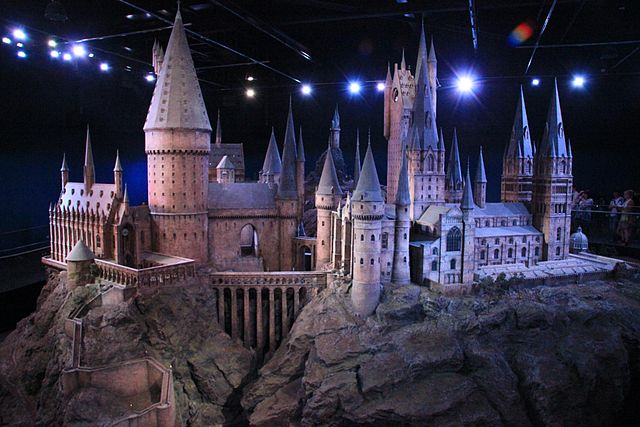
\includegraphics[width=.4\textwidth]{Hogwarts.jpg}
  \caption{An example figure\label{fig:example}}
\end{figure}

\section{Literature Review}

\lipsum[6] Table~\ref{tab:example} is an example table.

\begin{center}\singlespacing
  \captionof{table}{An example table\label{tab:example}}
  \begin{tabular}{lll}
    \toprule
    Name&School&Brief Info\\\midrule
    Harry Potter&Gryffindor&Good\\
    Draco Malfoy&Slytherin&Bad\\\bottomrule
  \end{tabular}
\end{center}


\section{Research Problem}
\lipsum[7]

\section{Objectives}
\lipsum[8]

\chapter{Materials}
\lipsum[9]
\section{Multidimensional Indices}
\lipsum[10]
\subsection{Data Collection}
\lipsum[11]
\subsubsection{Country Data}
\lipsum[12]

\subsubsection{Multidimensional Poverty Index (MPI)}
\lipsum[13]


\paragraph{National}
\lipsum[14]

\paragraph{Subnational}
\lipsum[15]

\section{Build Environment}
\lipsum[16]

\subsection{Google Colab}
\lipsum[17]

\subsection{Libraries}
\lipsum[18]

\chapter{Methodology}
\lipsum[19]

\section{Understanding the Data}
\lipsum[20]

\subsection{Data Distribution}
\lipsum[21]

\subsection{Data Preparation}
\lipsum[22]

\subsubsection{Data Cleaning}
\lipsum[23]

\subsubsection{Derived Metrics}
\lipsum[24]

\subsubsection{Feature Scaling}
\lipsum[25]

\subsection{Data Analytics}
\lipsum[26]

\subsubsection{Uni-variate Analysis}
\lipsum[27]

\subsubsection{Heatmap}
\lipsum[28]

\subsubsection{Pairplot}
\lipsum[29]

\section{Data Correlation Coefficients}
\lipsum[30]

\subsection{Pearson Correlation}
\lipsum[31]

\subsection{Kendall Correlation}
\lipsum[32]

\subsection{Spearman Correlation}
\lipsum[33]

\section{Principal Component Analysis (PCA) Application}
\lipsum[34]

\section{Hopkins Statistics Test}
\lipsum[35]

\section{Model Building}
\lipsum[36]

\subsection{K-Means Clustering}
\lipsum[37]

\subsection{Optimal Numbers of Clusters}
\lipsum[38]

\subsubsection{Elbow Method}
\lipsum[39]

\subsubsection{Silhouette Analysis}
\lipsum[40]

\subsection{Hierarchical Clustering}
\lipsum[41]

\subsubsection{Single Linkage}
\lipsum[42]

\subsubsection{Complete Linkage}
\lipsum[43]

\subsection{Cluster Analysis}
\lipsum[44]

\section{Final Analysis}
\lipsum[45]

\chapter{Conclusion}
\lipsum[46]

\section{Result}
\lipsum[47]

\section{Discussion}
\lipsum[48]

\appendix%

\makebib % Bibliography

\begin{advisorInfo} 
  WANG Xiaolin, obtained his MSc degree in distributed computing systems in Greenwich
  University, London, UK in 1998. Since 2004, he has been working as a lecturer in Southwest
  Forestry University teaching computer networks, operating systems, and Linux application
  programming related courses.  
\end{advisorInfo}

\begin{acknowledgment}
  Thank God, it's over!
\end{acknowledgment}

%%%%% Appendix chapters
\singlespacing

\chapter{Code Samples}

\section{C sample}

\lipsum[50]

\begin{ccode}
#include<stdio.h>

int main(void)
{
  printf("Hello, world!\n");
}
\end{ccode}

\section{Shell script example}

\lipsum[51]

\begin{shellcode}
  #!/bin/bash

  echo 'Hello, world!'
\end{shellcode}

\section{Python sample}

\lipsum[52]

\begin{pythoncode}
#!/usr/bin/python3

print("Hello, world!")
\end{pythoncode}

\end{document}
%%% Local Variables:
%%% mode: latex
%%% TeX-master: t
%%% End:
